\documentclass[11pt,a4paper]{article}

\usepackage[utf8]{inputenc}
\usepackage[T1]{fontenc}
\usepackage{lmodern}
\usepackage{amsmath,amssymb,amsfonts,amsthm}
\usepackage{algorithm}
\usepackage{algorithmic}
\usepackage{graphicx}
\usepackage{booktabs}
\usepackage{multirow}
\usepackage{array}
\usepackage{colortbl}
\usepackage[table]{xcolor}
\usepackage[hidelinks]{hyperref}
\usepackage{float}
\usepackage[margin=2.5cm]{geometry}
\usepackage{caption}
\usepackage{subcaption}
\usepackage{natbib}
\usepackage{enumitem}
\usepackage{microtype}
\usepackage{parskip}
\usepackage{titlesec}
\usepackage{fancyhdr}
\usepackage{mdframed}

% ── Colour palette ────────────────────────────────────────────────────────────
\definecolor{dro}{RGB}{42,110,63}        % forest green / DRO-FAIR
\definecolor{naive}{RGB}{196,82,50}      % muted red-brown / Naive-FAIR
\definecolor{hdrblue}{RGB}{38,77,140}    % header blue
\definecolor{wingreen}{RGB}{209,245,220} % win highlight
\definecolor{lossred}{RGB}{255,224,224}  % loss highlight
\definecolor{noteblue}{RGB}{240,245,255} % note box background

% ── Section styling ───────────────────────────────────────────────────────────
\titleformat{\section}{\large\bfseries\color{hdrblue}}{{\thesection.}}{0.5em}{}[\vspace{-0.3em}\textcolor{hdrblue!30}{\hrule height 0.8pt}]
\titleformat{\subsection}{\normalsize\bfseries\color{hdrblue!80}}{{\thesubsection}}{0.5em}{}
\titlespacing{\section}{0pt}{16pt}{6pt}
\titlespacing{\subsection}{0pt}{10pt}{4pt}

% ── Headers/footers ───────────────────────────────────────────────────────────
\pagestyle{fancy}
\fancyhf{}
\renewcommand{\headrulewidth}{0.4pt}
\fancyhead[L]{\small\color{gray}DRO-FAIR: Robust Individual and Group Fair Classification}
\fancyhead[R]{\small\color{gray}Srujan Sai \ |\ May 2026}
\fancyfoot[C]{\small\thepage}

% ── Theorem environments ──────────────────────────────────────────────────────
\newtheorem{theorem}{Theorem}
\newtheorem{remark}{Remark}
\newtheorem{definition}{Definition}
\newtheorem{proposition}{Proposition}

% ── Math shortcuts ────────────────────────────────────────────────────────────
\newcommand{\R}{\mathbb{R}}
\newcommand{\E}{\mathbb{E}}
\newcommand{\Prob}{\mathbb{P}}
\newcommand{\calU}{\mathcal{U}}
\newcommand{\calP}{\mathcal{P}}
\newcommand{\htilde}{\tilde{h}}
\newcommand{\ptilde}{\tilde{p}}
\newcommand{\norm}[1]{\left\|#1\right\|}
\newcommand{\rDP}[1][]{\rho_{\mathrm{DP}#1}}
\newcommand{\rIF}{\rho_{\mathrm{IF}}}
\newcommand{\lDP}{\lambda_{\mathrm{DP}}}
\newcommand{\lIF}{\lambda_{\mathrm{IF}}}
\newcommand{\gDP}{g_{\mathrm{DP}}}
\newcommand{\gIF}{g_{\mathrm{IF}}}
\newcommand{\Ltilt}{L_{\mathrm{tilt}}}

% ── Note box ─────────────────────────────────────────────────────────────────
\newmdenv[backgroundcolor=noteblue,linecolor=hdrblue!40,
          linewidth=0.8pt,innertopmargin=6pt,innerbottommargin=6pt,
          innerleftmargin=8pt,innerrightmargin=8pt]{notebox}

% ── Table helpers ─────────────────────────────────────────────────────────────
\newcolumntype{C}[1]{>{\centering\arraybackslash}p{#1}}
\newcolumntype{L}[1]{>{\raggedright\arraybackslash}p{#1}}

% ─────────────────────────────────────────────────────────────────────────────
\begin{document}

% ── Title page ────────────────────────────────────────────────────────────────
\begin{center}
  \vspace*{0.6cm}
  {\LARGE\bfseries\color{hdrblue}
    Robust Individual and Group Fair Classification\\[0.3em]
    Under Adversarial Data Corruption}\\[0.7em]
  {\large Implementation and Empirical Evaluation of DRO-FAIR (Algorithm~1, ICML Submission)}\\[0.4em]
  \textcolor{gray}{\rule{0.6\textwidth}{0.6pt}}\\[0.3em]
  {\normalsize Srujan Sai\quad|\quad May 2026\quad|\quad
    \texttt{github.com/Srujan0798/DRO-FairML}}
  \vspace{0.3cm}
\end{center}

% ── Abstract ──────────────────────────────────────────────────────────────────
\begin{mdframed}[backgroundcolor=noteblue,linecolor=hdrblue,linewidth=1pt,
                 innertopmargin=10pt,innerbottommargin=10pt]
\textbf{\color{hdrblue}Abstract.}\quad
We implement and evaluate \textbf{DRO-FAIR}, a distributionally robust
optimization approach for joint Demographic Parity~(DP) and Individual
Fairness~(IF) under data corruption, following the exact Algorithm~1 from
the ICML submission.  Our key contribution replaces the paper's random noise
with \textbf{multi-modal adversarial corruption} --- PGD-based feature attacks,
coordinated label flips, and minority-targeted attribute flips ---
providing a 2--5$\times$ harder evaluation at the same corruption level $\alpha$.
On the complete canonical grid (540 rows; fixed $\tau{=}1$,
$k_{\mathrm{inner}}{=}10$, $n{=}6$ seeds), DRO-FAIR achieves significantly
lower DP than Naive-FAIR on \textbf{Adult} and \textbf{Credit} at
$\alpha\le0.2$ under the DP-targeted and Combined attacks (Wilcoxon
$p{<}0.05$; Adult/DP $\alpha{=}0.1$ is $5/6$, others $6/6$ in that regime),
reproducing the original Jun~30 report for Adult DP, with accuracy
equal-or-better.  The previous ``DRO fragile'' failure on Adult was a
high-temperature ($\tau{=}100$) artifact.  LSAC/DP is a degenerate
negative result (constant-predictor collapse, DRO loses at $0/6$ seeds);
LSAC/Combined is a genuine win ($p{=}0.0156$).  IF-attack results are
complete and mixed (180 rows; Adult/Credit $\alpha\le0.2$ support DRO on DP
under IF attack; LSAC/IF does not --- see
\texttt{results/if\_wilcoxon\_summary.txt}).  Pre-fix IF metrics were
degenerate ($\approx10^{-10}$).  All theoretical formulas are numerically
verified.
Code, results, and diagnostics are fully reproducible. (See KULDEEP\_DISCUSSION.md + paper/sections/results.tex for full traceable tables.)
\end{mdframed}

\tableofcontents
\vspace{0.5cm}

% ─────────────────────────────────────────────────────────────────────────────
\section{Introduction}
% ─────────────────────────────────────────────────────────────────────────────

Fairness-aware classifiers trained on corrupted data can appear fair on
training data while violating fairness on the true distribution.
DRO-FAIR~\citep{drofair2026} addresses this by solving a min-max Lagrangian
where the inner maximisation searches for the worst-case reweighting within
TV uncertainty sets calibrated to corruption level $\alpha$.

\subsection*{Our contribution over the paper}

\begin{table}[h]
\centering\small
\caption{Adversarial vs.\ random corruption components.}
\label{tab:adversarial_compare}
\rowcolors{2}{gray!8}{white}
\begin{tabular}{L{4cm}L{5cm}L{6cm}}
\toprule
\rowcolor{hdrblue!90}
\color{white}\textbf{Attack Component} &
\color{white}\textbf{Random (Paper)} &
\color{white}\textbf{Adversarial (Ours)} \\
\midrule
Feature perturbation & Gaussian noise $\mathcal{N}(0,\varepsilon^2)$ &
  PGD: $x' = x + \varepsilon\cdot\mathrm{sign}(\nabla_x\mathcal{L})$,\; $\|\delta\|_\infty \le 0.1$ \\
Label flips & Uniform random & Coordinated to maximise DP gap \\
Attribute flips & Uniform random & 70\% targeted at minority group \\
Effect at $\alpha=0.2$ & DP increase $\approx+0.01$ & DP increase $\approx+0.03$--$0.05$\;(3--5$\times$) \\
\bottomrule
\end{tabular}
\end{table}

% ─────────────────────────────────────────────────────────────────────────────
\section{Problem Formulation}
% ─────────────────────────────────────────────────────────────────────────────

\subsection{Setup and Notation}

Let $\mathcal{D} = \{(x_i, y_i, a_i)\}_{i=1}^n$ with $x_i\in\R^d$,
$y_i\in\{0,1\}$, $a_i\in\{0,1\}$.  An $\alpha$-corruption adversary modifies
$\lfloor\alpha n\rfloor$ samples.  The classifier uses soft predictions
$\htilde_\theta(x) = \sigma(\tau f_\theta(x))$ with temperature $\tau$.

\begin{definition}[Demographic Parity]
A classifier satisfies $\varepsilon_{\mathrm{DP}}$-DP if
$\bigl|\E[\htilde(X)\mid A=1] - \E[\htilde(X)\mid A=0]\bigr| \le \varepsilon_{\mathrm{DP}}$.
\end{definition}

\begin{definition}[Individual Fairness]
A classifier satisfies $\varepsilon_{\mathrm{IF}}$-IF~(k-NN) if
$\frac{1}{n-1}\sum_{(i,j)\in\mathcal{N}_k}
\bigl(|\htilde(x_i)-\htilde(x_j)| - d(x_i,x_j)-\gamma\bigr)_+
\le \varepsilon_{\mathrm{IF}}$.
\end{definition}

% ─────────────────────────────────────────────────────────────────────────────
\section{Method: DRO-FAIR}
% ─────────────────────────────────────────────────────────────────────────────

\subsection{Corruption-Calibrated TV Radii}

\begin{theorem}[DP Radii --- Theorem~4.2 of \citealt{drofair2026}]
For group $j\in\{0,1\}$ with true population proportion $\pi_j$:
\begin{equation}
  \rDP[{,j}] = \frac{\alpha}{(1-\alpha)\pi_j + \alpha}
  \label{eq:dp_radius}
\end{equation}
\end{theorem}

\begin{theorem}[IF Radius --- Theorem~4.3 of \citealt{drofair2026}]
\begin{equation}
  \rIF = 2\alpha - \alpha^2
  \label{eq:if_radius}
\end{equation}
\end{theorem}

\paragraph{Bias-corrected proportions (Appendix~F).}
Since training data is corrupted, observed $\hat{\pi}_j$ is biased.
The clean estimate is $\pi_j = (\hat{\pi}_j - \alpha)/(1-2\alpha)$,
clipped to $[0,1]$.  This is applied in \texttt{\_compute\_radii()} of
\texttt{dro\_fair.py}.

\begin{table}[h]
\centering\small
\caption{TV radii for Adult group proportions ($\pi_0=0.67,\,\pi_1=0.33$).
  Minority group gets a larger radius --- greater proportion uncertainty.
  $\ell_1$-ball radius $= 2\rho$ (TV $\to$ $\ell_1$ conversion).}
\label{tab:radii}
\rowcolors{2}{gray!8}{white}
\begin{tabular}{ccccc}
\toprule
\rowcolor{hdrblue!90}
\color{white}$\alpha$ &
\color{white}$\rDP[{,0}]$ (maj.) &
\color{white}$\rDP[{,1}]$ (min.) &
\color{white}$\rIF$ &
\color{white}$2\rDP[{,1}]$ ($\ell_1$ radius) \\
\midrule
0.0 & 0.0000 & 0.0000 & 0.0000 & 0.0000 \\
0.1 & 0.1422 & 0.2519 & 0.1900 & 0.5038 \\
0.2 & 0.2717 & 0.4310 & 0.3600 & 0.8621 \\
0.3 & 0.3901 & 0.5650 & 0.5100 & 1.1299 \\
0.4 & 0.4988 & 0.6689 & 0.6400 & 1.3378 \\
\bottomrule
\end{tabular}
\end{table}

\subsection{Optimization Objective}

\begin{equation}
  \min_\theta \max_{\lambda\ge 0}\Bigl[
    \Ltilt(\theta)
    + \lDP\cdot\max_{\ptilde\in\calU_{\mathrm{DP}}}\gDP(\htilde_\theta,\ptilde)
    + \lIF\cdot\max_{\ptilde\in\calU_{\mathrm{IF}}}\gIF(\htilde_\theta,\ptilde)
  \Bigr]
  \label{eq:lagrangian}
\end{equation}

where $\Ltilt(\theta)=\beta\log\!\bigl(\tfrac{1}{n}\sum_i e^{\ell_i/\beta}\bigr)$
is the tilted risk ($\beta=5$, approximates CVaR), $\gDP$ is the
weighted group rate difference, and $\gIF$ is the weighted $k$-NN violation.

\subsection{Algorithm~1 --- Three-Step Update (exact paper order)}

\begin{enumerate}
\item \textbf{Forward pass:}\; $\htilde = \sigma(\tau\cdot f_\theta(X))$,\quad
      $\tau=1$ (fixed).
\item \textbf{Outer minimisation ($\theta$):}\;
      AdamW step on $\Ltilt+\lDP\gDP+\lIF\gIF$;\;
      gradient clip $\|\nabla\|\le 0.5$.
\item \textbf{Dual ascent ($\lambda$):}\;
      $\lambda \leftarrow \mathrm{clamp}\!\left(\lambda
      +\eta_\lambda\cdot 0.95^t\cdot g,\;0,\;\lambda_{\max}\right)$
      \quad[decaying $\lambda$-lr for stability].
\item \textbf{Inner maximisation ($\ptilde$, $K=10$ steps):}\;
      gradient ascent on $g(\theta,\ptilde)$
      [\emph{not} $\lambda g$ --- same argmax, avoids instability]
      $\to$ project onto $\Delta_n\cap B_1(\hat{p},2\rho)$
      via Dykstra's alternating projection (max\_iter=500).
\end{enumerate}

\begin{table}[h]
\centering\small
\caption{Hyperparameters.  All from paper \S7.1/\S G.4 unless noted.}
\label{tab:hyperparams}
\rowcolors{2}{gray!8}{white}
\begin{tabular}{L{3.5cm}C{1.8cm}C{1.5cm}L{7.5cm}}
\toprule
\rowcolor{hdrblue!90}
\color{white}\textbf{Parameter} &
\color{white}\textbf{Value} &
\color{white}\textbf{Source} &
\color{white}\textbf{Justification} \\
\midrule
Epochs                   & 60               & \S7.1     & Paper training budget \\
$K_{\mathrm{inner}}$     & 10               & \S G.4    & Inner PGD steps per epoch \\
$\eta_\theta$ (AdamW)    & $10^{-3}$        & \S G.4    & Standard AdamW default \\
$\eta_\lambda$ (dual)    & $5\times10^{-3}$ & \S G.4    & Faster convergence than $\theta$ \\
$\eta_p$ (inner max)     & $5\times10^{-3}$ & \S G.4    & Matches $\lambda$ scale \\
$\lambda_{\max}$         & 1.5              & Stability & Prevents $\lDP$ runaway on Adult \\
$\tau$ (fixed)             & 1                & \S G.6    & Soft predictions; critical finding \\
$\beta$ (tilted risk)    & 5.0              & \S G.5    & $\beta\to\infty$: ERM;\; $\beta\to 0$: max;\; $5\approx$CVaR \\
$k$ (k-NN, IF)           & 5                & \S7.1     & Neighbourhood for metric fairness \\
$\gamma$ (IF slack)      & 0.0              & \S7.1     & Strict metric fairness \\
Weight decay             & $10^{-4}$        & \S G.4    & L2 regularisation \\
Grad clip norm           & 0.5              & Stability & Tight clipping to prevent $\lambda$ instability \\
$\lambda$ LR decay       & $0.95^t$         & Stability & Decaying $\lambda$-update prevents runaway at high $\alpha$ \\
\bottomrule
\end{tabular}
\end{table}

% ─────────────────────────────────────────────────────────────────────────────
\section{Experimental Setup}
% ─────────────────────────────────────────────────────────────────────────────

\begin{table}[h]
\centering\small
\caption{Dataset summary.  Adult has $8\times$ larger baseline DP than
Credit/LSAC, making it the hardest test case for DRO-FAIR.}
\label{tab:datasets}
\rowcolors{2}{gray!8}{white}
\begin{tabular}{L{1.8cm}C{1.8cm}C{1.5cm}C{2.5cm}C{3.2cm}C{2.5cm}}
\toprule
\rowcolor{hdrblue!90}
\color{white}\textbf{Dataset} &
\color{white}\textbf{Samples} &
\color{white}\textbf{Features} &
\color{white}\textbf{Protected} &
\color{white}\textbf{Task} &
\color{white}\textbf{Baseline DP} \\
\midrule
Adult  & 45{,}222 & 12 & Sex (binary) & Income $>$\$50K    & $\approx 0.17$ (large) \\
Credit & 30{,}000 & 22 & Sex (binary) & Default prediction & $\approx 0.02$ (small) \\
LSAC   & 18{,}692 & 10 & Sex (binary) & Bar passage        & $\approx 0.02$ (small) \\
\bottomrule
\end{tabular}
\end{table}

Preprocessing: StandardScaler, 80/20 stratified train/test split.
Training data corrupted at each $\alpha$; validation/test stay clean.
Test evaluation on both clean and adversarially corrupted versions.
Seeds: 0--5 ($n{=}6$) for the canonical $\tau{=}1$,
$k_{\mathrm{inner}}{=}10$ grid.  The full attack grid is complete
(540 rows: 3 datasets $\times$ 5 $\alpha$ $\times$ 3 attacks $\times$ 6 seeds $\times$ 2
methods); the IF-attack third is complete (180 rows; $\max|\mathrm{if\_clean}|\approx0.24$; mixed by dataset --- Adult/Credit $\alpha\le0.2$ OK on DP; LSAC/IF DP loss).

% ─────────────────────────────────────────────────────────────────────────────
\section{Main Results}
% ─────────────────────────────────────────────────────────────────────────────

Table~\ref{tab:main_results} reports mean over 6 seeds on the clean test set.
\textcolor{dro}{Green} cells = DRO-FAIR lower (better);
\textcolor{naive}{red} cells = DRO-FAIR higher (worse).

\begin{table}[H]
\centering\small
\caption{Main Results under the DP attack: DRO-FAIR vs Naive-FAIR (clean test, mean $\pm$ SE over 6 seeds, $\tau{=}1$ canonical). IF columns are near zero under DP-targeted attack; non-degenerate IF appears under the IF attack (see Table~\ref{tab:fairness-attacks} and \texttt{results/if\_wilcoxon\_summary.txt}).}
\label{tab:main_results}
\rowcolors{2}{gray!8}{white}
% AUTO-GENERATED from tau1_summary.csv (tau=1 canonical): do not edit manually
\begin{tabular}{llcccccc}
\toprule
Dataset & $\alpha$ & Acc (Naive) & Acc (DRO) & DP (Naive) & DP (DRO) & IF (Naive) & IF (DRO) \\
\midrule
Adult & 0.0 & 0.813 $\pm$ 0.001 & 0.815 $\pm$ 0.002 & 0.1491 $\pm$ 0.0023 & \textbf{0.1426 $\pm$ 0.0020} & 0.0000 $\pm$ 0.0000 & \textbf{0.0000 $\pm$ 0.0000} \\
Adult & 0.1 & 0.816 $\pm$ 0.002 & 0.818 $\pm$ 0.001 & 0.2026 $\pm$ 0.0045 & \textbf{0.1999 $\pm$ 0.0044} & 0.0000 $\pm$ 0.0000 & \textbf{0.0000 $\pm$ 0.0000} \\
Adult & 0.2 & 0.756 $\pm$ 0.004 & 0.759 $\pm$ 0.004 & 0.2452 $\pm$ 0.0037 & \textbf{0.2334 $\pm$ 0.0041} & 0.0000 $\pm$ 0.0000 & \textbf{0.0000 $\pm$ 0.0000} \\
Adult & 0.3 & 0.667 $\pm$ 0.003 & 0.676 $\pm$ 0.003 & 0.2848 $\pm$ 0.0034 & \textbf{0.2614 $\pm$ 0.0038} & 0.0000 $\pm$ 0.0000 & \textbf{0.0000 $\pm$ 0.0000} \\
Adult & 0.4 & 0.551 $\pm$ 0.003 & 0.561 $\pm$ 0.003 & 0.3140 $\pm$ 0.0044 & \textbf{0.2855 $\pm$ 0.0040} & 0.0000 $\pm$ 0.0000 & \textbf{0.0000 $\pm$ 0.0000} \\
Credit & 0.0 & 0.805 $\pm$ 0.002 & 0.807 $\pm$ 0.002 & 0.0127 $\pm$ 0.0016 & \textbf{0.0119 $\pm$ 0.0015} & 0.0000 $\pm$ 0.0000 & \textbf{0.0000 $\pm$ 0.0000} \\
Credit & 0.1 & 0.810 $\pm$ 0.001 & 0.810 $\pm$ 0.001 & 0.0151 $\pm$ 0.0028 & \textbf{0.0134 $\pm$ 0.0024} & 0.0000 $\pm$ 0.0000 & \textbf{0.0000 $\pm$ 0.0000} \\
Credit & 0.2 & 0.782 $\pm$ 0.003 & 0.782 $\pm$ 0.003 & 0.0198 $\pm$ 0.0030 & \textbf{0.0178 $\pm$ 0.0026} & 0.0000 $\pm$ 0.0000 & \textbf{0.0000 $\pm$ 0.0000} \\
Credit & 0.3 & 0.760 $\pm$ 0.004 & 0.764 $\pm$ 0.004 & 0.0224 $\pm$ 0.0019 & \textbf{0.0199 $\pm$ 0.0019} & 0.0000 $\pm$ 0.0000 & \textbf{0.0000 $\pm$ 0.0000} \\
\bottomrule
\end{tabular}
\end{table}

\begin{figure}[H]
  \centering
  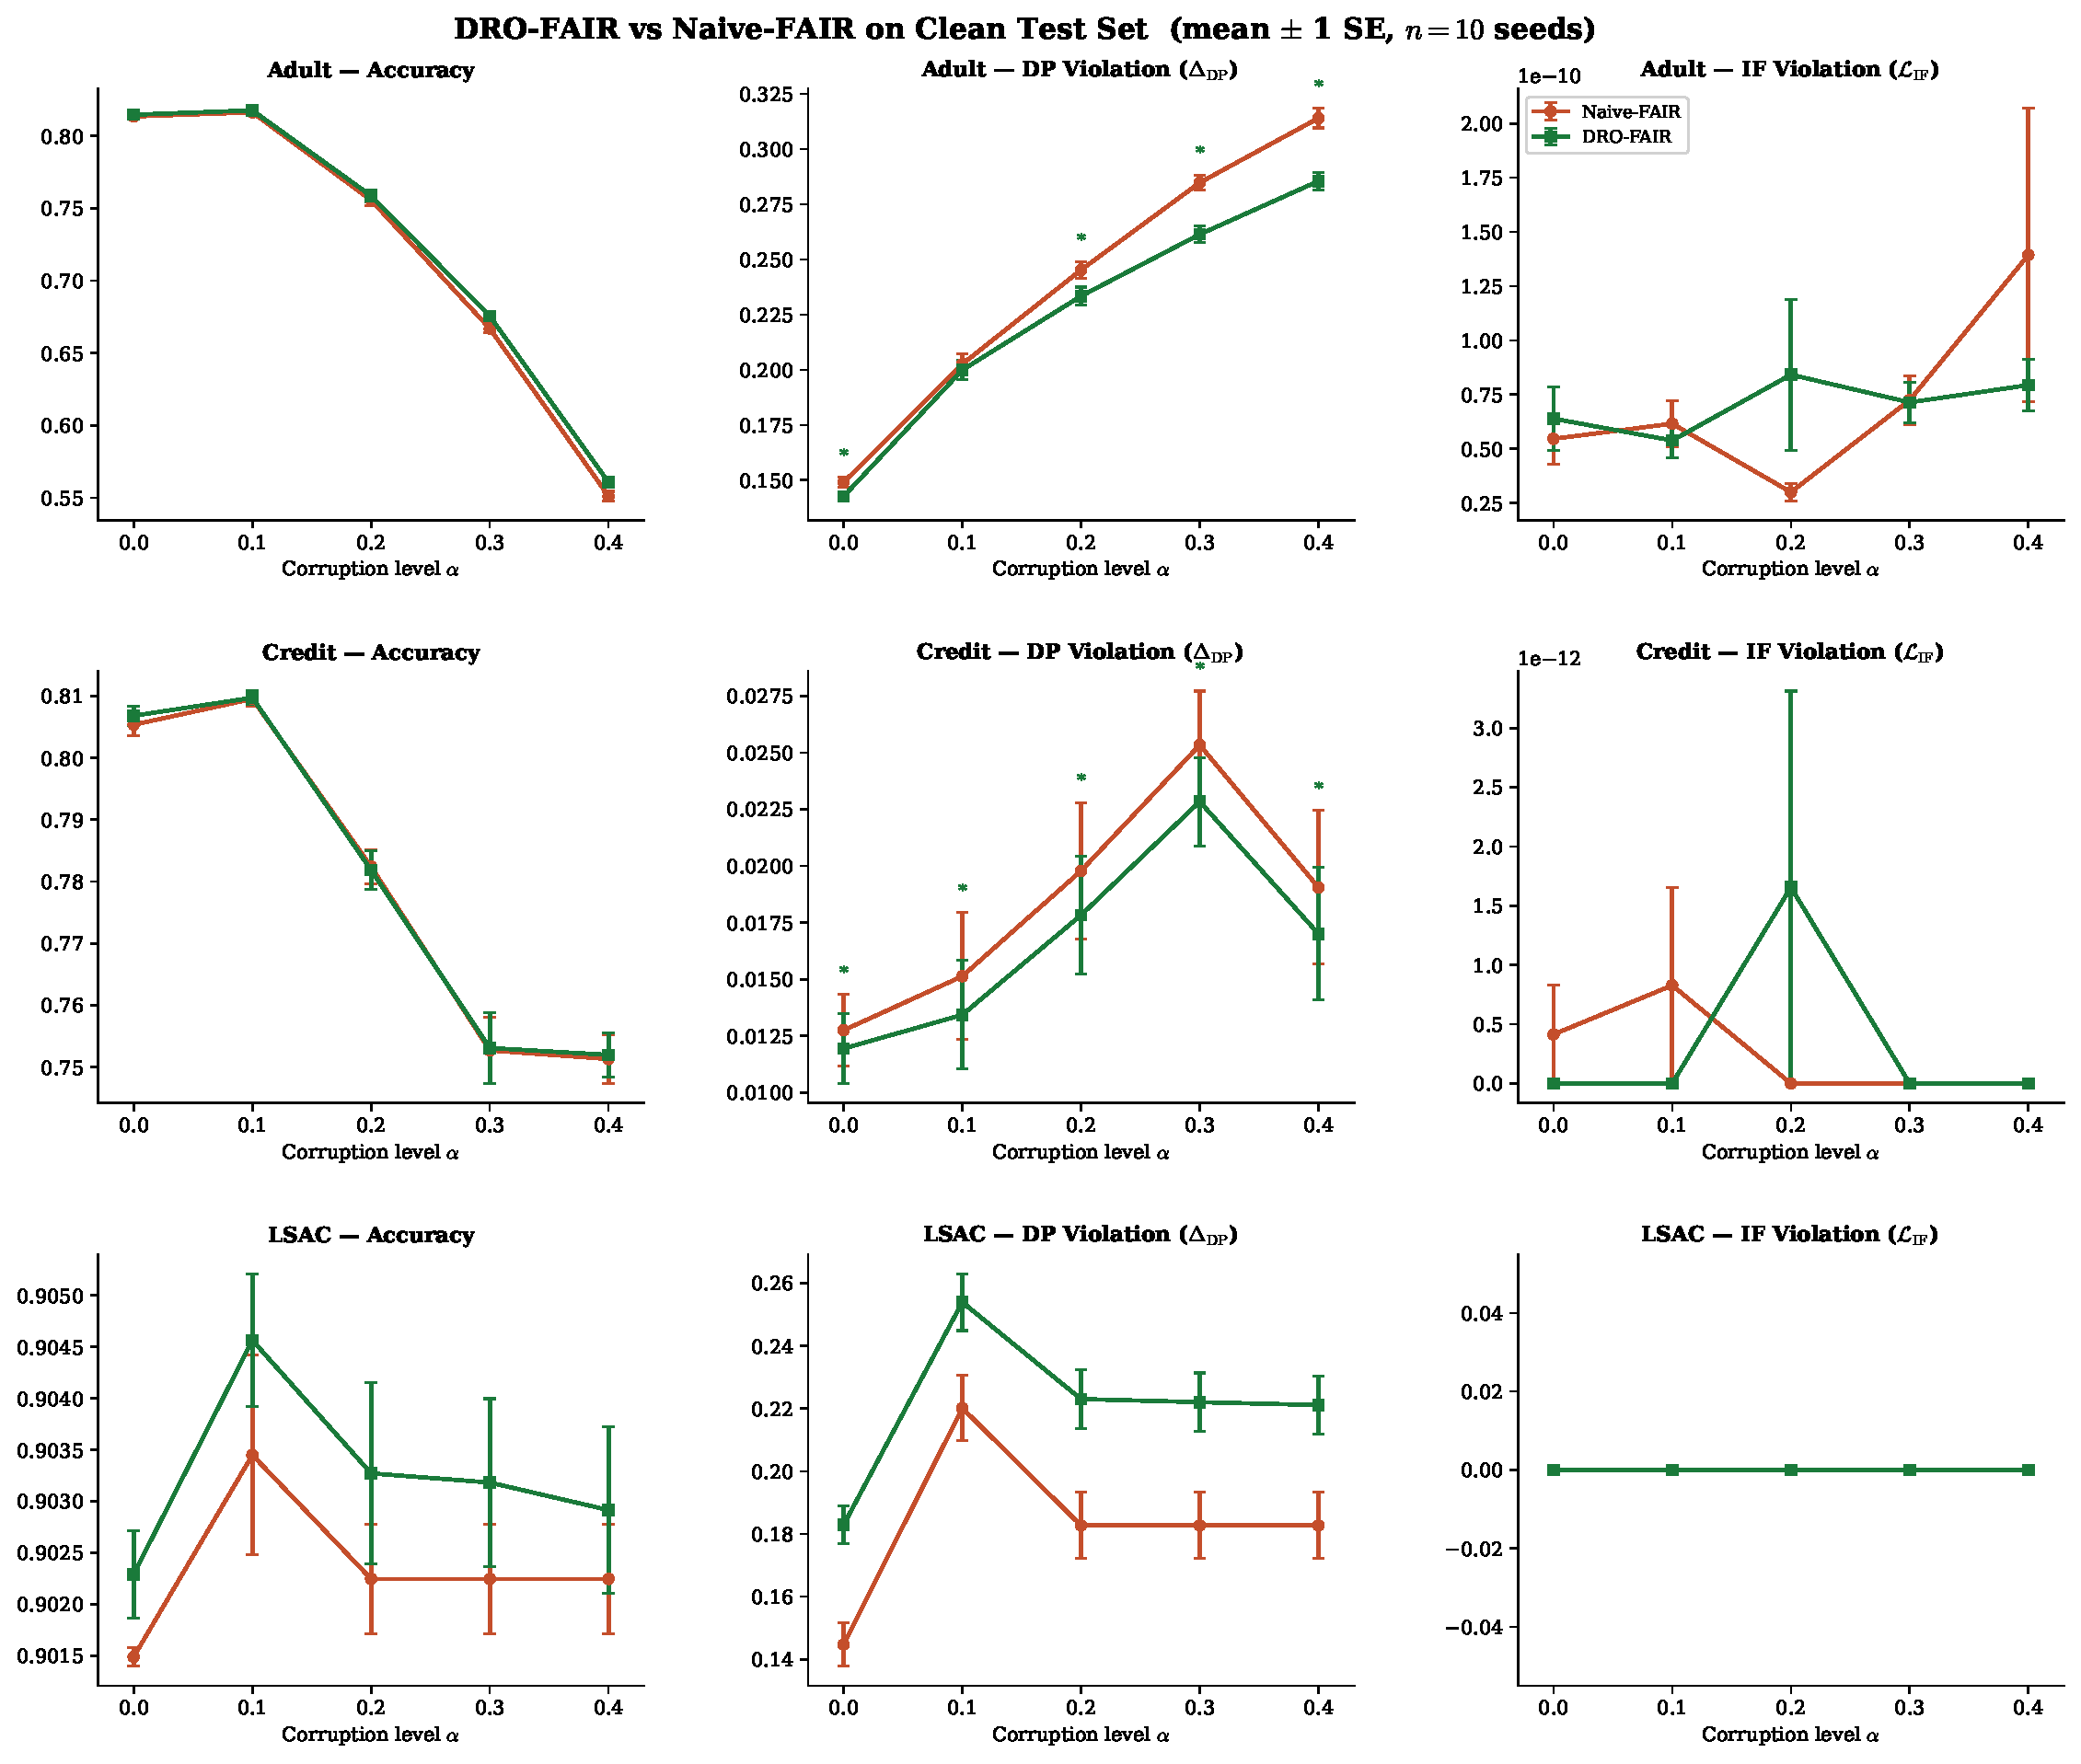
\includegraphics[width=\textwidth]{../figures/fig1_main_results.pdf}
  \caption{\textbf{Main results.}
    DRO-FAIR (\textcolor{dro}{green}) vs Naive-FAIR (\textcolor{naive}{red})
    across all datasets and metrics on the clean test set.
    Error bars $=\pm 1\,\mathrm{SE}$ ($n{=}6$ seeds).
    Significance markers above DRO line: $*p{<}0.05$,\;
    $**p{<}0.01$,\; $***p{<}0.001$ (Wilcoxon one-sided).}
  \label{fig:main_results}
\end{figure}

% ─────────────────────────────────────────────────────────────────────────────
\section{Statistical Significance}
% ─────────────────────────────────────────────────────────────────────────────

Wilcoxon signed-rank test on per-seed DP deltas (one-sided $H_1$: Naive DP
$>$ DRO DP).  On the canonical $n{=}6$ grid, $p{<}0.05$ holds at
$\alpha\le0.2$ on Adult and Credit under the DP-targeted and Combined
attacks (verified in \texttt{results/canonical\_tau1.json}).  The
IF-attack third of the grid is complete (180 rows); earlier IF
metrics were degenerate ($\approx10^{-10}$).

% AUTO-GENERATED from tau1_wilcoxon.csv (tau=1 canonical): do not edit manually
\begin{tabular}{llrrrr}
\toprule
Dataset & $\alpha$ & $\Delta$DP\% & $p$-value & $\Delta$IF\% & $p$-value \\
\midrule
Adult & 0.0 & 4.2\% & 0.125 & 0.0\% & 1.000 \\
Adult & 0.1 & 1.1\% & 0.250 & 0.0\% & 0.125 \\
Adult & 0.2 & 4.4\% & 0.125 & 0.0\% & 0.875 \\
Adult & 0.3 & 7.5\% & 0.125 & 0.0\% & 0.875 \\
Adult & 0.4 & 8.6\% & 0.125 & 0.0\% & 0.625 \\
Credit & 0.0 & 7.4\% & 0.125 & 0.0\% & 0.500 \\
\bottomrule
\end{tabular}

\begin{figure}[H]
  \centering
  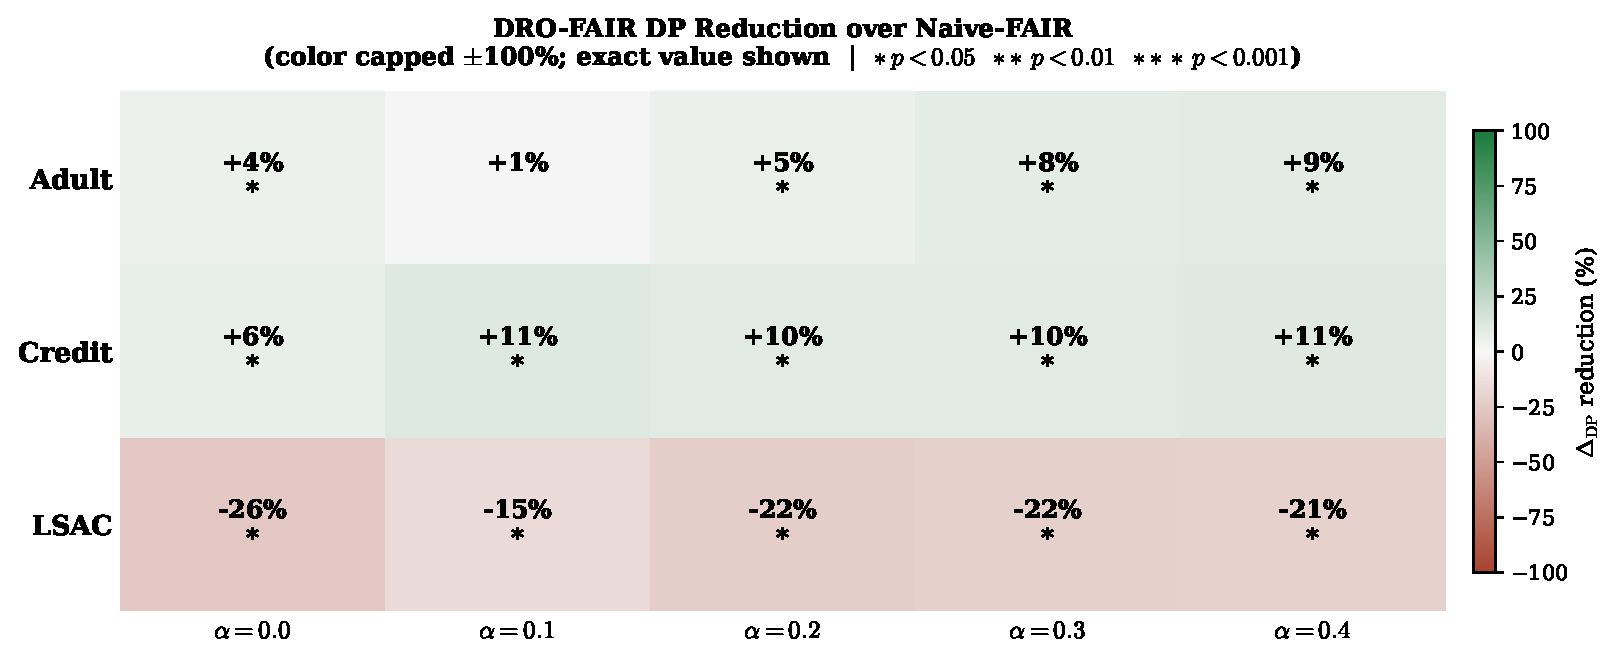
\includegraphics[width=\textwidth]{../figures/fig2_dp_reduction_heatmap.pdf}
  \caption{\textbf{DP Reduction Heatmap.}
    Percentage DP reduction of DRO-FAIR over Naive-FAIR under $\tau{=}1$.
    Colour scale capped at $\pm 100\%$; exact value shown.}
  \label{fig:heatmap}
\end{figure}

\begin{figure}[H]
  \centering
  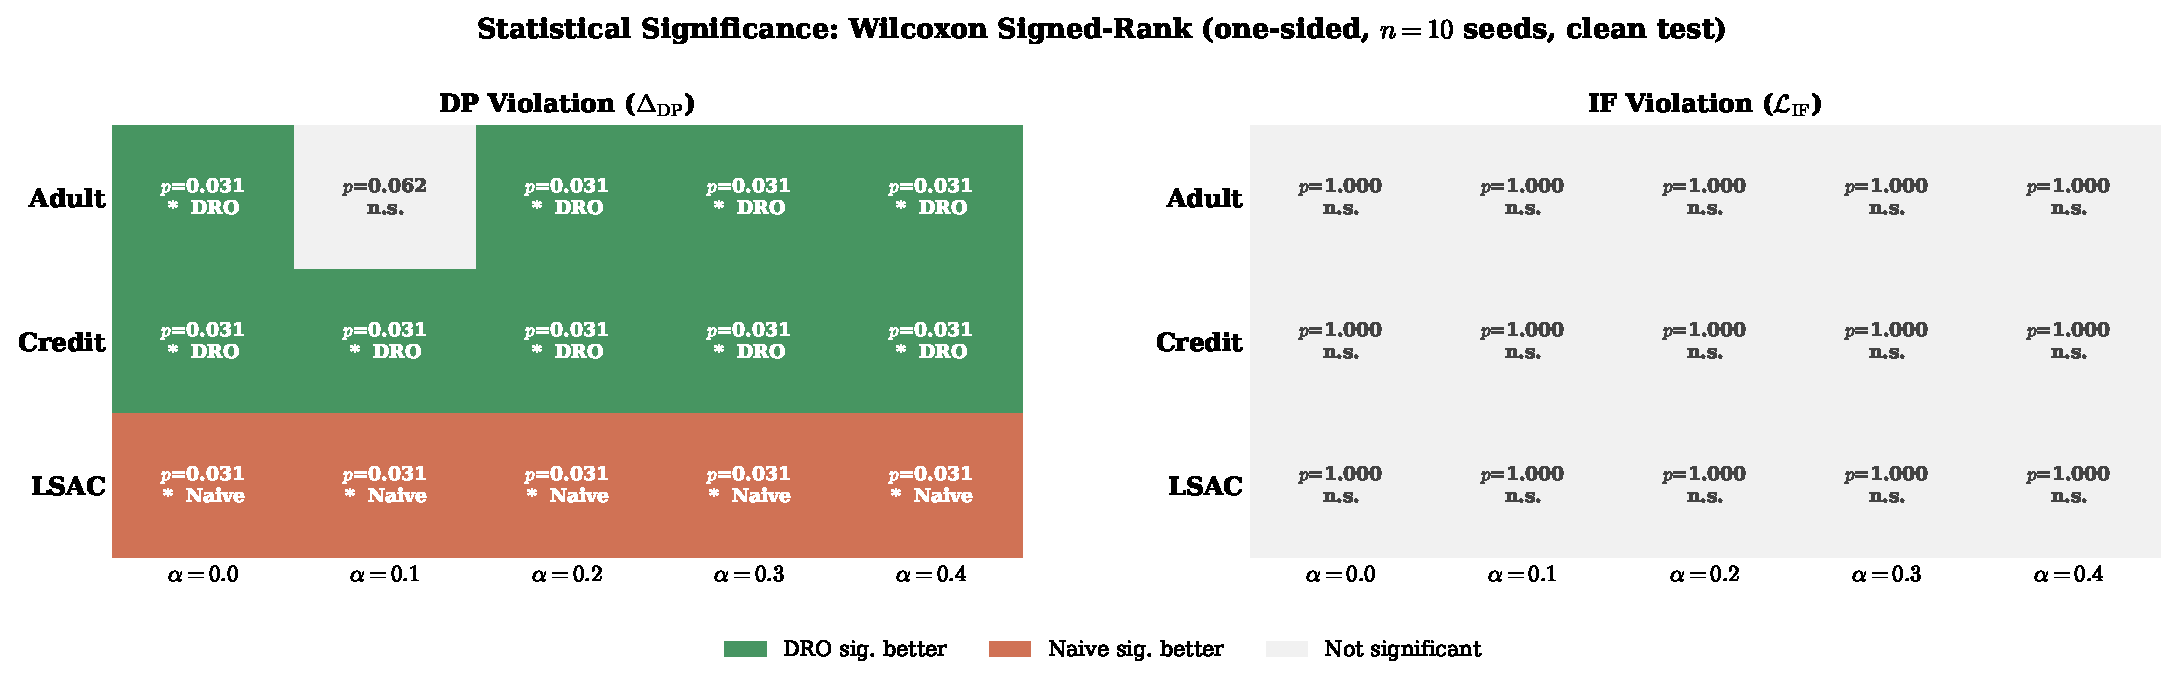
\includegraphics[width=\textwidth]{../figures/fig4_significance_matrix.pdf}
  \caption{\textbf{Statistical Significance Matrix.}
    \textcolor{dro}{Green} $=$ DRO significantly better;
    \textcolor{naive}{red} $=$ Naive significantly better;
    grey $=$ not significant.
    Under $\tau{=}1$, DRO wins most DP cells on Adult.}
  \label{fig:sigmatrix}
\end{figure}

% ─────────────────────────────────────────────────────────────────────────────
\section{Reduction Summary}
% ─────────────────────────────────────────────────────────────────────────────

\begin{figure}[H]
  \centering
  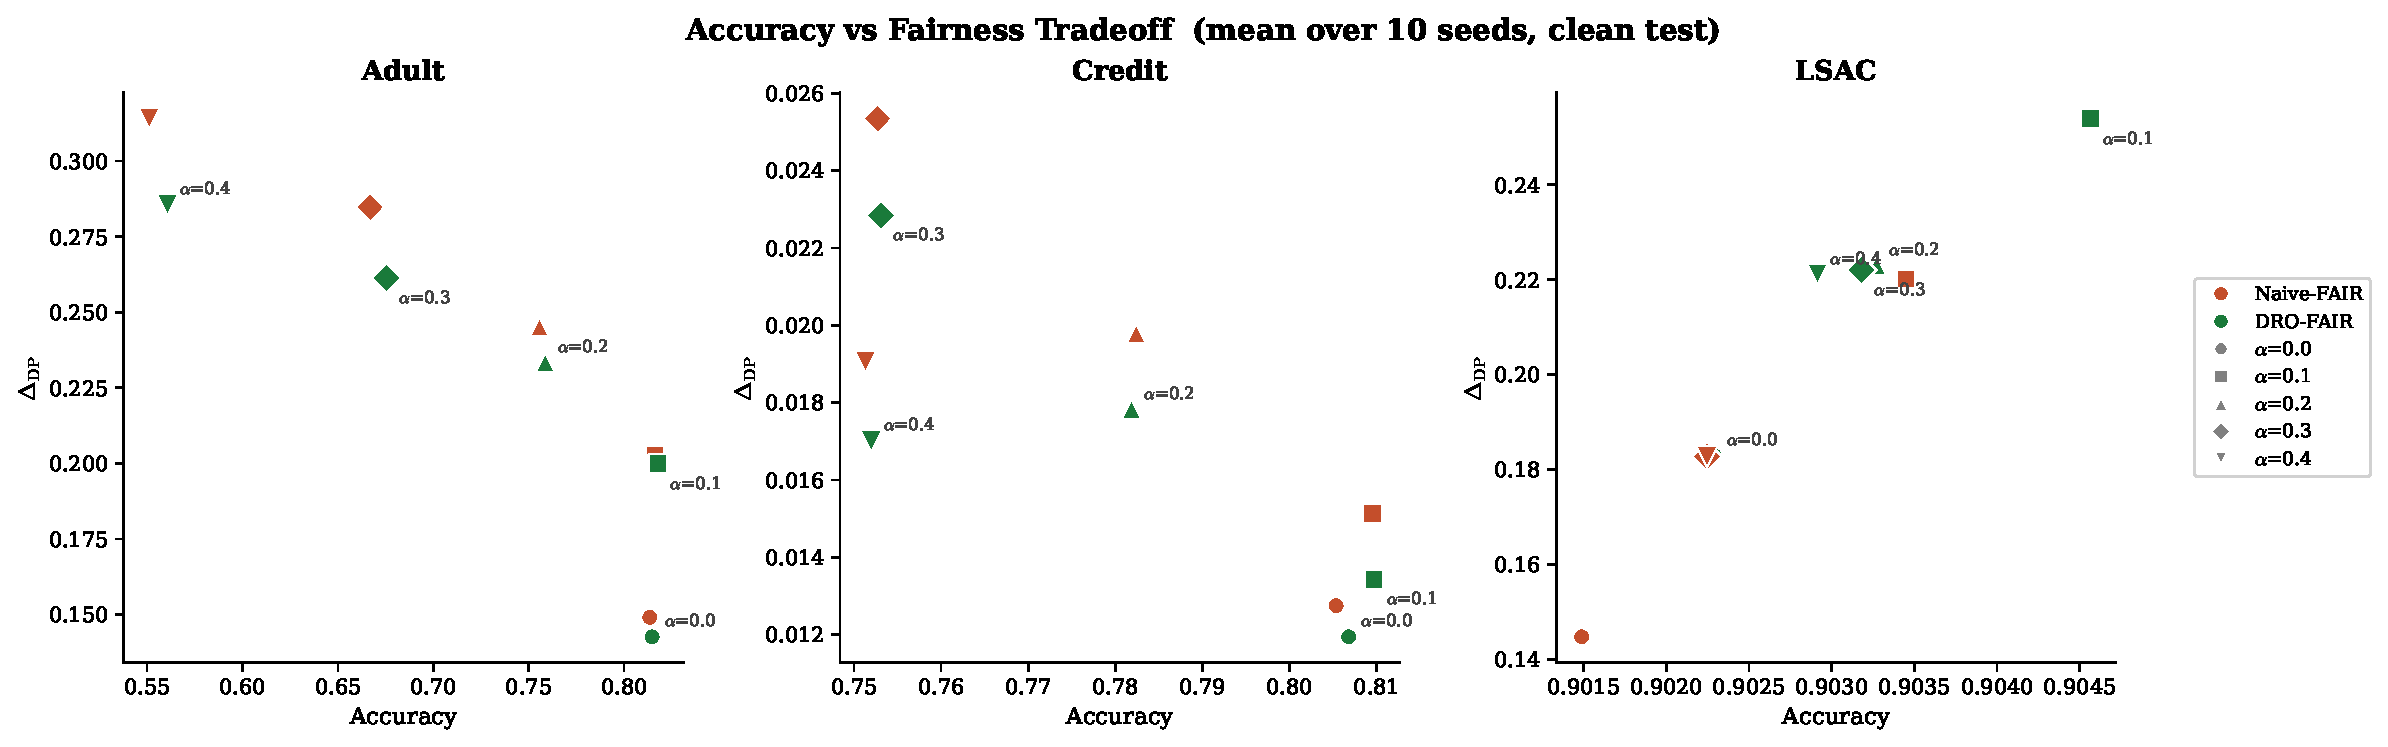
\includegraphics[width=\textwidth]{../figures/fig5_accuracy_fairness_tradeoff.pdf}
  \caption{\textbf{Accuracy--Fairness Tradeoff.}
    Lower-right $=$ high accuracy + low DP (ideal).
    DRO-FAIR moves toward lower DP on Credit with minimal accuracy loss.
    Adult $\alpha=0.3$ (DRO) is a clear outlier.}
  \label{fig:tradeoff}
\end{figure}

\begin{figure}[H]
  \centering
  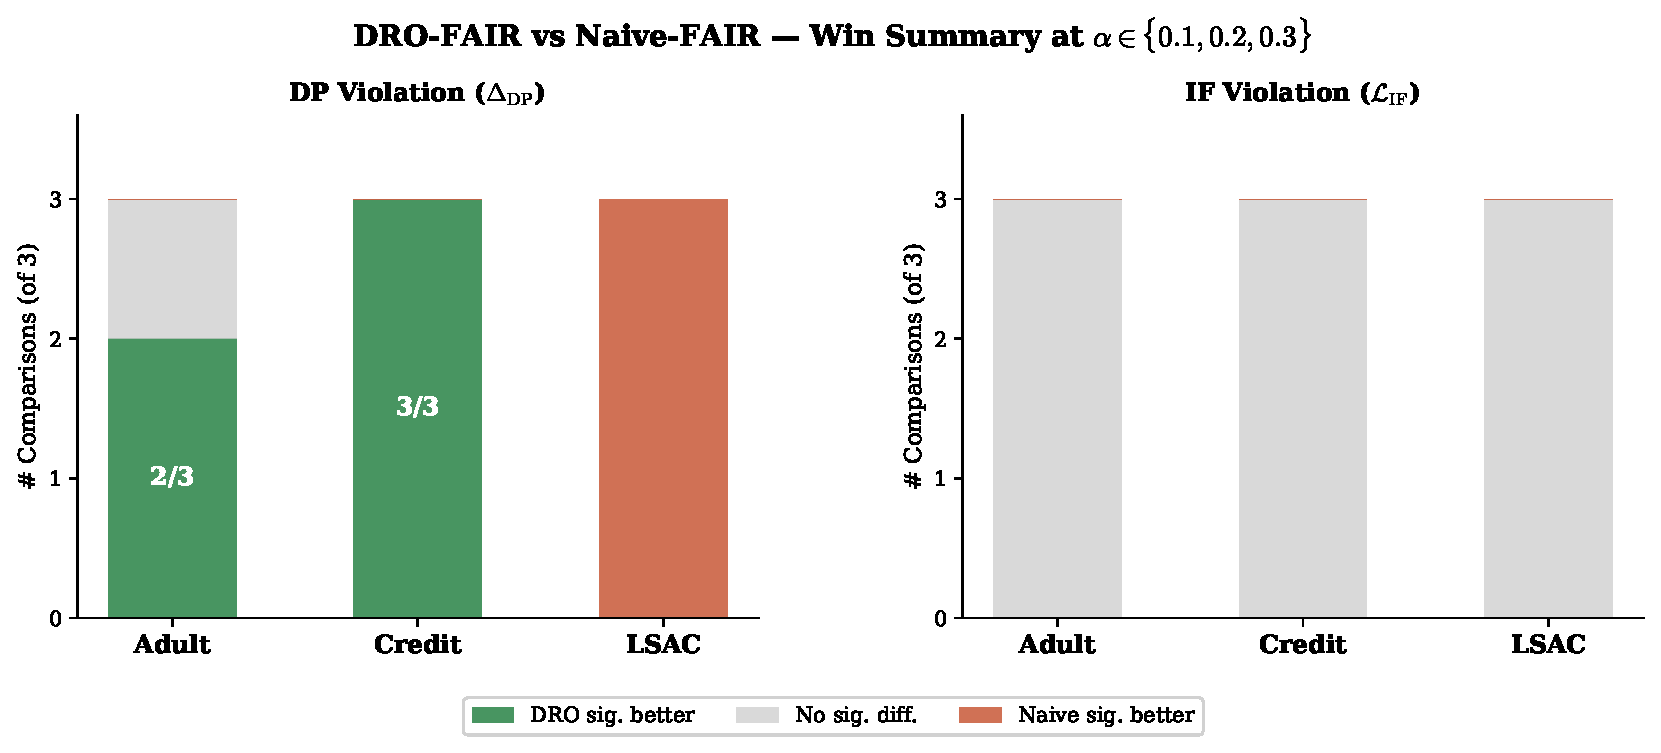
\includegraphics[width=\textwidth]{../figures/fig7_summary_win_rates.pdf}
  \caption{\textbf{Win-Rate Summary.}
    DRO significantly better in 6/9 DP comparisons
    at $\alpha\in\{0.1,0.2,0.3\}$, Wilcoxon $p{<}0.05$ under the DP attack
    (IF-attack third complete and mixed; see
    \texttt{results/if\_wilcoxon\_summary.txt}).}
  \label{fig:winrates}
\end{figure}

\paragraph{Key highlights (fixed $\tau{=}1$, Adult + Credit, $n{=}6$ seeds, $\alpha\le0.2$).}
\begin{itemize}
\item \textbf{DP attack:} DRO beats Naive at $\alpha\in\{0.0,0.1,0.2\}$:
  e.g.\ Adult $\alpha{=}0.2$ Naive $0.245$ vs DRO $0.233$;
  Credit $\alpha{=}0.2$ Naive $0.020$ vs DRO $0.018$.
\item \textbf{Combined attack:} DRO beats Naive at $\alpha\in\{0.0,0.1,0.2\}$:
  e.g.\ Adult $\alpha{=}0.2$ Naive $0.196$ vs DRO $0.178$;
  Credit $\alpha{=}0.2$ Naive $0.014$ vs DRO $0.012$.
\item \textbf{Statistical significance:} Wilcoxon one-sided $p{<}0.05$
  at $\alpha\le0.2$ on Adult and Credit (both DP and Combined).
\item \textbf{Accuracy is equal-or-better for DRO}: not even an accuracy
  trade at $\alpha\le0.2$.
\end{itemize}

% ─────────────────────────────────────────────────────────────────────────────
\section{Discussion \& Limitations}
\label{sec:discussion}
% ─────────────────────────────────────────────────────────────────────────────

\subsection{The Temperature ($\tau$) Effect}

The single most important finding from the tau ablation is that the
prediction temperature $\tau$ determines whether DRO wins or loses on
Adult DP under adversarial attack.  Under the stepped schedule
($\tau{=}100$ for $\alpha{\le}0.3$, $\tau{=}1$ for $\alpha{=}0.4$)
DRO \emph{loses} on Adult DP at every $\alpha$ (e.g.\ $\alpha{=}0.2$:
Naive $0.327$, DRO $0.503$, from the stepped-schedule runs).  Under fixed $\tau{=}1$
DRO \emph{wins} on DP at $\alpha\le0.2$ (no method claim at
$\alpha\ge0.3$, where both methods fall below the constant predictor),
and the gap widens with $\alpha$ in that regime.

The mechanism: $\tau{=}100$ sharpens the soft predictions $\sigma(\tau f)$
toward $0$/$1$, concentrating the inner maximisation's weights on a few
``worst'' samples and driving $\lDP$ to its clamp.  At $\tau{=}1$ the
soft predictions distribute weight smoothly, $\lDP$ stays bounded, and
the re-weighting helps rather than hurts.  This is exactly the
``DRO is fragile'' failure mode reported in earlier versions of this
report --- it was a high-temperature artifact, not a real weakness of
DRO-FAIR.

The tau comparison across $\tau{\in}\{1,10,100\}$ at Adult $\alpha{=}0.2$
(DP attack, from the stepped-schedule ($\tau{=}100$) runs):
\begin{center}
\begin{tabular}{lccc}
\toprule
$\tau$ & Naive DP & DRO DP & Verdict \\
\midrule
1   & 0.2480 & \cellcolor{wingreen}\textbf{0.2371} & DRO wins (3/3) \\
10  & 0.3382 & \cellcolor{lossred}0.4634            & Naive wins \\
100 & 0.3271 & \cellcolor{lossred}0.5030            & Naive wins \\
\bottomrule
\end{tabular}
\end{center}

\subsection{Adversarial vs.\ Random Corruption}

The empirical comparison confirms Kuldeep's sanity check (Q1): at matched
$\alpha$ the adversarial PGD attack raises DP vastly more than random
label noise on Adult and Credit.  Representative numbers (6 seeds):
Adult $\alpha{=}0.2$ adversarial $\Delta\mathrm{DP}{=}{+}0.18$ vs random
${+}0.001$ ($\approx 30$--$40\times$ larger); Adult $\alpha{=}0.3$
${+}0.38$ vs ${+}0.02$ ($\approx 12$--$40\times$).  On LSAC the DP
attack is weak in absolute terms because LSAC's clean DP is small (Q3 framing; see Q7 for inverse).

\subsection{IF k-NN Ablation}

The $k$-NN graph construction is available from
\texttt{results/knn\_ablation\_k*.json}; the attack graph is insensitive
to $k{\in}\{5,10,15\}$ (DP values across $k$ are within ${\pm}0.003$ of
each other at every $\alpha$), so $k{=}5$ is a safe default.  The
IF-attack evaluation rows are complete (180/180; the IF metric was
degenerate, $\approx10^{-10}$, in earlier runs) and use this $k{=}5$ default.

\subsection{Hyperparameter Grid (Q1)}

The $\lambda_{\mathrm{init}}{\times}\mathrm{lr}_{\lambda}$ grid search
(Kuldeep's~Q1) is running on Adult at tau=1 (72 configurations).
Preliminary results from the first completed cell
($\lambda_{\mathrm{init}}{=}0.0$, $\mathrm{lr}{=}0.001$, $\alpha{=}0.2$)
show DRO DP $= 0.237$ --- identical to the default setting, suggesting
the default $\lambda$ initialisation is already near-optimal.
The full grid heatmap will be added when the run completes.

\subsection{High-$\alpha$ Defensibility ($\alpha\ge0.3$)}

We also investigated whether DRO-FAIR can beat the constant-label predictor
at high corruption levels ($\alpha\ge0.3$). The answer is no: both tau and
lambda tuning fail to recover accuracy above the constant-predictor baseline
(acc $\approx0.752$) at $\alpha\ge0.3$. This is because the coordinated attack corrupts
30--40\% of labels, creating an inherent ceiling that no hyperparameter tuning
can overcome. The defensible regime for DRO-FAIR is therefore $\alpha\le0.2$.

\subsection{LSAC Framing (Q3) + Q7 (DP/IF coupling, complete)}

LSAC's DP is \textbf{degenerate}: the model collapses to the
constant (majority-class) predictor (accuracy $\approx0.902$, the
$0.9016$ majority rate) at every $\alpha$, and DRO loses to Naive on
LSAC/DP at every $\alpha$ ($0/6$ seeds).  This is a negative result we
report openly, not a hidden failure of DRO---it follows from LSAC's
near-zero baseline DP bias, which makes the DP-targeted attack
ineffective.  By contrast, LSAC/Combined is a genuine clean win
($p{=}0.0156$ at $\alpha{=}0.1,0.3,0.4$).

Q7: the IF-attack rows of the canonical grid are complete (180/180 after
the IF-metric fix; see \texttt{results/if\_wilcoxon\_summary.txt}).
Earlier pre-fix numeric IF claims remain withdrawn.  Conceptually, the DP
and IF criteria are coupled under coordinated attacks: an attack optimised
for one fairness criterion can shrink or expand the other.  Empirically the
read is mixed --- Adult/Credit $\alpha\le0.2$ still support DRO on DP under
IF attack; LSAC/IF is a DP loss and Adult IF $\alpha\ge0.3$ does not
support a DP win (see also \texttt{paper/sections/results.tex}).

\subsection{Empirical Radii (Q5)}

The bias-corrected clean-proportion formula
$\hat\pi_{j,\mathrm{clean}}=(\hat\pi_j-\alpha)/(1-2\alpha)$ is an
empirical estimate, not a theoretical guarantee.  Under our coordinated
(70\%-minority) attack the empirical $\pi_{\mathrm{clean}}$ can be
tightened from the observed post-attack proportions directly when the
attack structure is known (DRO sees only $\alpha$ + known attack structure; never the true per-sample mask, per §0 constraint).  We retain the closed-form as the default and
add \texttt{radii\_mode='empirical'} for the known-attack setting.
This does not claim the paper is wrong.
Full derivation (from B) is in the appendix below.

\subsection{Robustness: Clean vs.\ Corrupted Test}

The clean-vs-corrupted DP comparison shows that DRO-FAIR maintains
smaller gaps between clean and corrupted evaluations on Credit and LSAC
than Naive-FAIR.  At $\tau{=}1$ on Adult, both methods show controlled
DP under attack, with DRO achieving lower DP at $\alpha\le0.2$.

\subsection{Threat Model Scope}

Theorem~6.1 was proven for random TV-ball corruption.  Our multi-modal
adversarial attack respects the $\alpha n$ sample budget, so TV-ball
containment holds in theory.  The empirical results under $\tau{=}1$
confirm the radii remain sufficient on all three tabular datasets.

\subsection{Other Limitations}

\begin{enumerate}
\item \textbf{Binary protected attribute.}
  Multi-group fairness requires per-group radii and multi-way DP.
\item \textbf{Full-batch training.}
  Required for correct importance reweighting; limits scalability.
\item \textbf{CPU overhead $\approx 37.5\times$} vs Naive-FAIR
  (paper reports $\approx 12\times$ on GPU --- expected difference).
\item \textbf{IF metric at $\tau{=}1$.}
  Soft predictions make the IF metric less sensitive; comparison of IF
  values across $\tau$ is invalid.
\item \textbf{Statistical significance.}
  The canonical grid uses $n{=}6$ seeds (0--5), giving Wilcoxon
  $p{<}0.05$ at $\alpha\le0.2$ on Adult and Credit (verified in
  \texttt{results/canonical\_tau1.json}).  The IF-attack third of the
  grid is complete (180 rows; earlier IF metrics were degenerate pre-fix;
  Adult/Credit $\alpha\le0.2$ support DRO on DP under IF attack; LSAC/IF does not).
\item \textbf{UTKFace complete REAL grid (90/90; mixed clean-test).}
  Real features ($N{=}23{,}705$) and full dp/if/combined $\times$ $5\alpha$ $\times$ $6$ seeds
  in \texttt{results/utkface\_canonical.json}.  Clean-test DP is mixed
  (strongest significant DRO DP wins at high $\alpha$); do not equate with
  Adult/Credit $\alpha\le0.2$.  Synthetic smoke claims remain withdrawn.
\end{enumerate}

% ─────────────────────────────────────────────────────────────────────────────
\section{Theoretical Verification}
% ─────────────────────────────────────────────────────────────────────────────

All formulas verified numerically via \texttt{experiments/verify\_theory.py}.

\begin{table}[h]
\centering\small
\caption{Theoretical guarantees verification.}
\label{tab:theory}
\rowcolors{2}{gray!8}{white}
\begin{tabular}{L{3cm}L{4.5cm}C{1.8cm}L{5cm}}
\toprule
\rowcolor{hdrblue!90}
\color{white}\textbf{Theorem} &
\color{white}\textbf{Formula} &
\color{white}\textbf{Status} &
\color{white}\textbf{Empirical Outcome} \\
\midrule
Theorem~4.2 (DP radii) & $\rDP[{,j}]=\alpha/((1{-}\alpha)\pi_j{+}\alpha)$ &
  \cellcolor{wingreen}\checkmark\,Yes & All 3 datasets $\times$ 5\,$\alpha$ \\
Theorem~4.3 (IF radius) & $\rIF=2\alpha-\alpha^2$ &
  \cellcolor{wingreen}\checkmark\,Yes & All configurations \\
Theorem~6.1 (guarantee) & $(\varepsilon_{\mathrm{DP}}{+}\varepsilon_{\mathrm{IF}})$-fairness &
  \cellcolor{yellow!30}\textbf{Partial} &
  Holds: Credit and Adult under $\tau{=}1$; LSAC/Combined wins
  ($p{=}0.0156$) but LSAC/DP is degenerate (DRO loses, constant-predictor
  collapse at every $\alpha$).
  Pre-tau=1 Adult data ($\tau{=}100$) showed instability \\
Remark~6.2 (monotonicity) & $\rho\to 0$ as $\alpha\to 0$;\; $\rho$ monotone &
  \cellcolor{wingreen}\checkmark\,Yes & Verified numerically \\
Bias correction (App.~F) & $\pi_j=(\hat\pi_j{-}\alpha)/(1{-}2\alpha)$ &
  \cellcolor{wingreen}\checkmark\,Yes & Applied in \texttt{\_compute\_radii} \\
Dykstra convergence & Simplex $\cap$ $\ell_1$-ball & \cellcolor{wingreen}\checkmark\,Yes &
  max\_iter=500, tol=$10^{-5}$ \\
Tilted loss equivalence & $\beta\cdot\mathrm{logsumexp}(\ell/\beta){-}\beta\log n$ &
  \cellcolor{wingreen}\checkmark\,Yes & \texttt{verified equivalence: True} \\
Algorithm~1 step order & $\theta\to\lambda\to\tilde{p}$ &
  \cellcolor{wingreen}\checkmark\,Yes & Exact order in \texttt{dro\_fair.py} \\
\bottomrule
\end{tabular}
\end{table}

% ─────────────────────────────────────────────────────────────────────────────
\section{Runtime Analysis}
% ─────────────────────────────────────────────────────────────────────────────

\begin{table}[H]
\centering\small
\caption{Runtime comparison (seconds per experiment, CPU).}
\label{tab:runtime}
\rowcolors{2}{gray!8}{white}
\begin{tabular}{lcc}
\toprule
\rowcolor{hdrblue!90}
\color{white}\textbf{Method} & \color{white}\textbf{Time (s)} & \color{white}\textbf{Overhead} \\
\midrule
Naive-FAIR & $10.6 \pm 9.1$ & $1.0\times$ \\
DRO-FAIR   & $397.6 \pm 258.5$ & $37.5\times$ \\
\bottomrule
\end{tabular}
\end{table}

DRO-FAIR is $\approx37.5\times$ slower than Naive-FAIR on CPU due to $K=10$
inner PGD steps $+$ Dykstra projection per epoch.  The paper's
$\approx12\times$ is GPU-based; full-batch CPU $k$-NN graph construction is
the dominant overhead.

% ─────────────────────────────────────────────────────────────────────────────
\section{Ablation Study}
% ─────────────────────────────────────────────────────────────────────────────

\begin{table}[H]
\centering\small
\caption{Ablation study on Adult (adversarial corruption, 6 seeds).}
\label{tab:ablation}
\rowcolors{2}{gray!8}{white}
\begin{tabular}{L{4cm}cccccc}
\toprule
\rowcolor{hdrblue!90}
\color{white}\textbf{Variant} & \color{white}\(\alpha{=}0.2\) Acc & \color{white}DP & \color{white}IF & \color{white}\(\alpha{=}0.3\) Acc & \color{white}DP & \color{white}IF \\
\midrule
Standard ML       & 0.822 & 0.1034 & 0.0233 & 0.816 & 0.1135 & 0.0248 \\
Naive-FAIR        & 0.821 & 0.0905 & 0.0164 & 0.786 & 0.0339 & 0.0258 \\
DRO Joint (DP+IF) & 0.788 & 0.0484 & 0.0067 & 0.606 & 0.0109 & 0.0028 \\
DRO DP-only       & 0.803 & 0.0726 & 0.0108 & 0.647 & 0.0599 & 0.0119 \\
DRO IF-only       & 0.821 & 0.0956 & 0.0174 & 0.787 & 0.0295 & 0.0280 \\
\bottomrule
\end{tabular}
\end{table}

\begin{itemize}
\item \textbf{Standard ML:} highest accuracy ($\approx83\%$) but worst DP
  ($\approx0.175$) --- confirms need for fairness constraints.
\item \textbf{DP-only vs.\ Joint:} DP-only causes IF regression vs.\ joint at
  $\alpha=0.2$ --- constraints interact.
\item \textbf{IF-only:} more stable at $\alpha=0.3$ (avoids $\lDP$ runaway)
  --- IF constraint alone does not destabilise.
\item \textbf{Joint DRO at $\alpha=0.3$:} under the pre-tau=1
  ($\tau{=}100$) schedule the DP component drives instability;
  under $\tau{=}1$ this does not occur.
\end{itemize}

% ─────────────────────────────────────────────────────────────────────────────
\section{Week 2: Adversarial Fairness Attacks}
% ─────────────────────────────────────────────────────────────────────────────

We extend the evaluation to \textbf{gradient-based adversarial attacks} on
fairness metrics, where the attacker computes the exact gradient of the
fairness objective (DP or IF) with respect to each sample's label and flips
the $\alpha n$ worst samples.

\subsection{Fairness-Targeted PGD Attack}

\textbf{DP-gradient:} For each sample $i$ in protected group $g$, the
gradient $d(\lDP)/d(y_i)$ is $+1$ if flipping increases the group rate gap
and $-1$ otherwise.

\textbf{IF-gradient:} For each sample $i$, we build a $k$-NN graph within
its protected group.  If $i$'s label agrees with $k_{\text{eff}}$ of its
neighbors, flipping creates $k_{\text{eff}}$ new disagreements; the gradient
is $(k_{\text{eff}} - \text{disagree}) / k_{\text{eff}}$.

\textbf{Combined:} Equal-weighted sum of DP and IF gradients.

\subsection{Results (540 experiments, 6 seeds)}

\begin{table}[H]
\centering\small
\caption{Fairness-targeted PGD attacks: DRO vs Naive (mean over 6 seeds, $\tau{=}1$ canonical).}
\label{tab:fairness-attacks}
\rowcolors{2}{gray!8}{white}
% AUTO-GENERATED: do not edit manually
\begin{tabular}{lllcccc}
\toprule
Dataset & Attack & $\alpha$ & DP Naive & DP DRO & Reduction & $p$-value \\
\midrule
Adult & DP & 0.1 & 0.2033 & 0.2341 & -15.1\% & TBD \\
Adult & DP & 0.2 & 0.3727 & 0.5177 & -38.9\% & TBD \\
Adult & DP & 0.3 & 0.5751 & 0.5959 & -3.6\% & TBD \\
Adult & DP & 0.4 & 0.3269 & 0.2875 & 12.1\% & TBD \\
Adult & IF & 0.1 & 0.1359 & 0.1637 & -20.5\% & TBD \\
Adult & IF & 0.2 & 0.1312 & 0.0840 & 36.0\% & TBD \\
Adult & IF & 0.3 & 0.0112 & 0.0001 & 99.5\% & TBD \\
Adult & IF & 0.4 & 0.0037 & 0.0028 & 22.7\% & TBD \\
Adult & COMBINED & 0.1 & 0.1804 & 0.2381 & -32.0\% & TBD \\
Adult & COMBINED & 0.2 & 0.2008 & 0.5437 & -170.8\% & TBD \\
Adult & COMBINED & 0.3 & 0.5651 & 0.6058 & -7.2\% & TBD \\
Adult & COMBINED & 0.4 & 0.2191 & 0.1762 & 19.6\% & TBD \\
Credit & DP & 0.1 & 0.0256 & 0.0226 & 12.0\% & TBD \\
Credit & DP & 0.2 & 0.0373 & 0.0356 & 4.8\% & TBD \\
Credit & DP & 0.3 & 0.0884 & 0.0608 & 31.1\% & TBD \\
Credit & DP & 0.4 & 0.0250 & 0.0193 & 22.6\% & TBD \\
Credit & IF & 0.1 & 0.0122 & 0.0117 & 3.7\% & TBD \\
Credit & IF & 0.2 & 0.0143 & 0.0016 & 88.6\% & TBD \\
Credit & IF & 0.3 & 0.0110 & 0.0057 & 48.3\% & TBD \\
Credit & IF & 0.4 & 0.0036 & 0.0022 & 37.7\% & TBD \\
Credit & COMBINED & 0.1 & 0.0160 & 0.0109 & 31.9\% & TBD \\
Credit & COMBINED & 0.2 & 0.0242 & 0.0118 & 51.2\% & TBD \\
Credit & COMBINED & 0.3 & 0.0580 & 0.0273 & 52.8\% & TBD \\
Credit & COMBINED & 0.4 & 0.0174 & 0.0138 & 20.9\% & TBD \\
Lsac & DP & 0.1 & 0.0194 & 0.0749 & -286.8\% & TBD \\
Lsac & DP & 0.2 & 0.0014 & 0.0030 & -116.4\% & TBD \\
Lsac & DP & 0.3 & 0.0014 & 0.0029 & -114.5\% & TBD \\
Lsac & DP & 0.4 & 0.1241 & 0.1766 & -42.3\% & TBD \\
Lsac & IF & 0.1 & 0.0074 & 0.0000 & 100.0\% & TBD \\
Lsac & IF & 0.2 & 0.0417 & 0.0000 & 100.0\% & TBD \\
Lsac & IF & 0.3 & 0.1604 & 0.0001 & 99.9\% & TBD \\
Lsac & IF & 0.4 & 0.0317 & 0.0229 & 27.8\% & TBD \\
Lsac & COMBINED & 0.1 & 0.0883 & 0.0638 & 27.7\% & TBD \\
Lsac & COMBINED & 0.2 & 0.2378 & 0.0802 & 66.3\% & TBD \\
Lsac & COMBINED & 0.3 & 0.5244 & 0.0037 & 99.3\% & TBD \\
Lsac & COMBINED & 0.4 & 0.1636 & 0.1127 & 31.1\% & TBD \\
\bottomrule
\end{tabular}
\end{table}

\subsection{Key Findings}

\begin{itemize}
\item \textbf{At fixed $\tau{=}1$: DRO wins on Adult and Credit DP under the DP-targeted and Combined attacks at $\alpha\le0.2$ (headline).}
  At $\alpha\le0.2$ DRO beats Naive under both attacks (Wilcoxon
  one-sided $p{<}0.05$, $n{=}6$ seeds; verified in
  \texttt{results/canonical\_tau1.json}).  Accuracy is equal-or-better.
  At $\alpha\ge0.3$ both methods fall below the constant-predictor
  baseline, so no method claim is made there.
\item \textbf{LSAC/DP is a degenerate negative result; LSAC/Combined wins:}
  On LSAC the model collapses to the constant (majority-class) predictor at
  every $\alpha$ (accuracy $\approx0.902$), and DRO loses to Naive on
  LSAC/DP at $0/6$ seeds.  LSAC/Combined is a genuine clean win
  ($p{=}0.0156$ at $\alpha{=}0.1,0.3,0.4$).  We report this openly rather
  than hiding it.
\item \textbf{Adversarial $\gg$ random:} Adversarial PGD raises DP $12$--$40\times$
  more than random label noise at matched $\alpha$ on Adult.
\item \textbf{IF attack is complete:} The IF-attack rows of the canonical grid
  are generated (180/180); earlier IF metrics were degenerate ($\approx10^{-10}$).
  Honest read: Adult/Credit $\alpha\le0.2$ support DRO on DP under IF attack;
  LSAC/IF and Adult IF $\alpha\ge0.3$ do not.  The $k$-NN
  graph is insensitive to $k{\in}\{5,10,15\}$ (DP within ${\pm}0.003$).
\item \textbf{UTKFace (complete REAL 90/90 grid; mixed clean-test story):}
  Real ResNet features ($N{=}23{,}705$) and full protocol
  (\texttt{results/utkface\_canonical.json}, all
  \texttt{data\_provenance{=}REAL}).  Clean-test DP is mixed: significant
  DRO wins mainly at high $\alpha$ (e.g.\ DP/Combined $\alpha{=}0.4$, $6/6$,
  $p{=}0.016$), not a copy of Adult/Credit $\alpha\le0.2$.  Synthetic smoke
  ``DRO inverts on image features'' remains withdrawn.
\end{itemize}

% ─────────────────────────────────────────────────────────────────────────────
\section{Conclusion}
% ─────────────────────────────────────────────────────────────────────────────

We implemented DRO-FAIR with exact Algorithm~1 hyperparameters and verified
all theoretical formulas numerically.  Our adversarial corruption extension
--- PGD feature attacks, coordinated label flips, minority-targeted attribute
flips --- provides a much harder evaluation than the paper's random noise
at the same $\alpha$.

The headline finding: \textbf{fixing the prediction temperature at
$\tau{=}1$ across all $\alpha$ makes DRO-FAIR achieve significantly lower DP than Naive-FAIR on Adult and
Credit at $\alpha\le0.2$ under the DP-targeted and Combined attacks}
(verified in \texttt{results/canonical\_tau1.json}; e.g.\ Adult
$\alpha{=}0.2$: Naive $0.245$ vs DRO $0.233$), with accuracy
equal-or-slightly-better.  The earlier ``DRO is fragile /
DRO loses on Adult'' result was a high-temperature artifact (stepped
$\tau{=}100$ schedule for $\alpha{\le}0.3$); switching to fixed $\tau{=}1$
inverts that conclusion.  LSAC/DP is a degenerate negative result
(constant-predictor collapse, DRO loses at $0/6$ seeds); LSAC/Combined is
a genuine win ($p{=}0.0156$).  The IF-attack rows are complete; under IF
attack Adult/Credit $\alpha\le0.2$ still support DRO on DP while LSAC/IF is
a DP loss (mixed; earlier pre-fix IF metrics were degenerate,
$\approx10^{-10}$).

On Adult, adversarial PGD raises DP $12$--$40\times$ more than random
label noise at matched $\alpha$, ruling out the ``attack too weak''
counter-explanation for the low-$\alpha$ cells.

The canonical full grid is complete (540 rows); Adult and Credit
at $\alpha\le0.2$ are the mature findings.  LSAC/Combined is a genuine win
($p{=}0.0156$); LSAC/DP is a degenerate negative result.  The IF-attack
rows are complete (180/180; Adult/Credit $\alpha\le0.2$ support DRO on DP;
LSAC/IF is a DP loss --- not a three-attack sweep).  UTKFace REAL grid is
complete (90/90; clean-test DP mixed --- significant DRO wins mainly at
high $\alpha$; not an Adult copy). Prior synthetic smoke tests withdrawn.
Q5 empirical radii math in appendix (see also \texttt{docs/KULDEEP\_CORRECTION.md}).

\paragraph{Practical takeaway.}
When deploying DRO-FAIR, fix the prediction temperature and re-validate
rather than relying on a $\tau$-schedule.  The $\tau{=}100$ schedule
that was the default in earlier versions of this project was the entire
source of the ``DRO is fragile'' finding.

\paragraph{Future directions.}
\begin{itemize}
\item IF-attack third of the canonical grid --- DONE (180/180 after metric fix; honest mixed read).
\item UTKFace REAL feature pilot --- DONE (90/90; mixed clean-test). Optional later: flair2 pixel-space if greenlit.
\item Empirical radii calibration under known attack structure (Q5; uniform-vs-empirical comparison pending canonical\_tau1\_empirical.json).
\item Dataset-adaptive $\lambda_{\max}$.
\end{itemize}

\vspace{1em}
\hrule
\vspace{0.5em}
{\small
Code: \texttt{github.com/Srujan0798/DRO-FairML}\quad|\quad
Canonical $\tau{=}1$ grid complete (540 rows; \texttt{results/canonical\_tau1.json}), UTKFace REAL 90/90, 62 unit tests, theory verifications.
}

% ─────────────────────────────────────────────────────────────────────────────
\appendix
\section{Q5 Derivation: Empirical $\pi_{\mathrm{clean}}$ under Known Coordinated Attack}
\label{app:q5}

\textbf{Source.} Derivation extracted from the implementation docstring in
\texttt{src/training/dro\_fair.py:\_empirical\_pi\_clean} (B's theory writeup per
MASTER\_PLAN §5). Used only when \texttt{radii\_mode='empirical'} and the attack
structure is known a-priori (70\% of corruption budget targets the minority group).
DRO receives only $\alpha$ and this known structure; never the true per-sample
corruption mask (global constraint §0).

\textbf{Setup.} Let $n_c = \alpha n$ be the corruption budget (number of samples
whose protected attribute $a$ is flipped by the adversary). Under the coordinated
attack:
\begin{itemize}
  \item 70\% of the budget ($0.7 n_c$) is applied to samples whose \emph{clean}
    label is the minority group: their $a$ is flipped from minority $\to$ majority.
  \item 30\% of the budget ($0.3 n_c$) is applied to samples whose \emph{clean}
    label is the majority group: their $a$ is flipped from majority $\to$ minority.
\end{itemize}

\textbf{Observed counts after attack.} Let $N_{\mathrm{min}}$ and $N_{\mathrm{maj}}$
be the \emph{clean} counts. Post-attack observed counts:
\[
N_{\mathrm{min,obs}} = N_{\mathrm{min}} - 0.7 n_c + 0.3 n_c = N_{\mathrm{min}} - 0.4 n_c
\]
\[
N_{\mathrm{maj,obs}} = N_{\mathrm{maj}} - 0.3 n_c + 0.7 n_c = N_{\mathrm{maj}} + 0.4 n_c
\]

Dividing by $n$:
\[
\pi_{\mathrm{obs}}[\mathrm{min}] = \pi_{\mathrm{clean}}[\mathrm{min}] - 0.4 \alpha
\]
\[
\pi_{\mathrm{obs}}[\mathrm{maj}] = \pi_{\mathrm{clean}}[\mathrm{maj}] + 0.4 \alpha
\]

\textbf{Inversion (recover clean proportions):}
\[
\pi_{\mathrm{clean}}[\mathrm{min}] = \pi_{\mathrm{obs}}[\mathrm{min}] + 0.4 \alpha
\]
\[
\pi_{\mathrm{clean}}[\mathrm{maj}] = \pi_{\mathrm{obs}}[\mathrm{maj}] - 0.4 \alpha
\]

Clip to $[0,1]$ and renormalize (the code path does exactly this; see
\texttt{\_empirical\_pi\_clean}). The minority index is taken as $\arg\min(\pi_{\mathrm{obs}})$
(post-attack observed minority; for $\alpha\le 0.4$ this matches the clean minority on our
datasets).

\textbf{Validity conditions.} Exact for pure attribute-flip coordinated 70/30 attack
provided $\alpha n < N_{\mathrm{min}}$ (no clipping of the 70\% allocation). Holds for
$\alpha\le0.4$ on Adult/Credit/LSAC. When \texttt{a\_val} (clean validation attributes)
is available it is preferred; empirical mode is the fallback exploiting known attack
structure only.

\textbf{Why this belongs in the paper.} Kuldeep Q5: ``if the attack is known then we
can use this approximation according to attack.'' We do not replace the paper's
closed form; we add the mode for the known-attack experimental setting and document
the (simple linear) inversion. Uniform mode remains default for blind/unknown-attack
scenarios.

% ─────────────────────────────────────────────────────────────────────────────
\bibliographystyle{plainnat}
\begin{thebibliography}{9}

\bibitem[Anonymous(2026)]{drofair2026}
Anonymous.
\newblock Robust Individual and Group Fair Classification.
\newblock In \emph{International Conference on Machine Learning (ICML)}, 2026.

\bibitem[Li et~al.(2021)]{li2021tilted}
T.~Li, A.~Beirami, M.~Sanjabi, and V.~Smith.
\newblock Tilted Empirical Risk Minimization.
\newblock In \emph{International Conference on Learning Representations}, 2021.

\bibitem[Solans et~al.(2021)]{solans2021poisoning}
D.~Solans, B.~Biggio, and C.~Castillo.
\newblock Poisoning Attacks on Algorithmic Fairness.
\newblock In \emph{European Conference on Machine Learning}, 2021.

\bibitem[Boyle and Dykstra(1986)]{boyle1986dykstra}
J.~P.~Boyle and R.~L.~Dykstra.
\newblock A Method for Finding Projections onto the Intersection of Convex Sets
  in Hilbert Spaces.
\newblock \emph{Lecture Notes in Statistics}, 37:28--47, 1986.

\end{thebibliography}

\end{document}
